%\documentclass{article}
%\usepackage{graphicx,subfigure}
%\begin{document}

\begin{figure}[h]
  \centering
  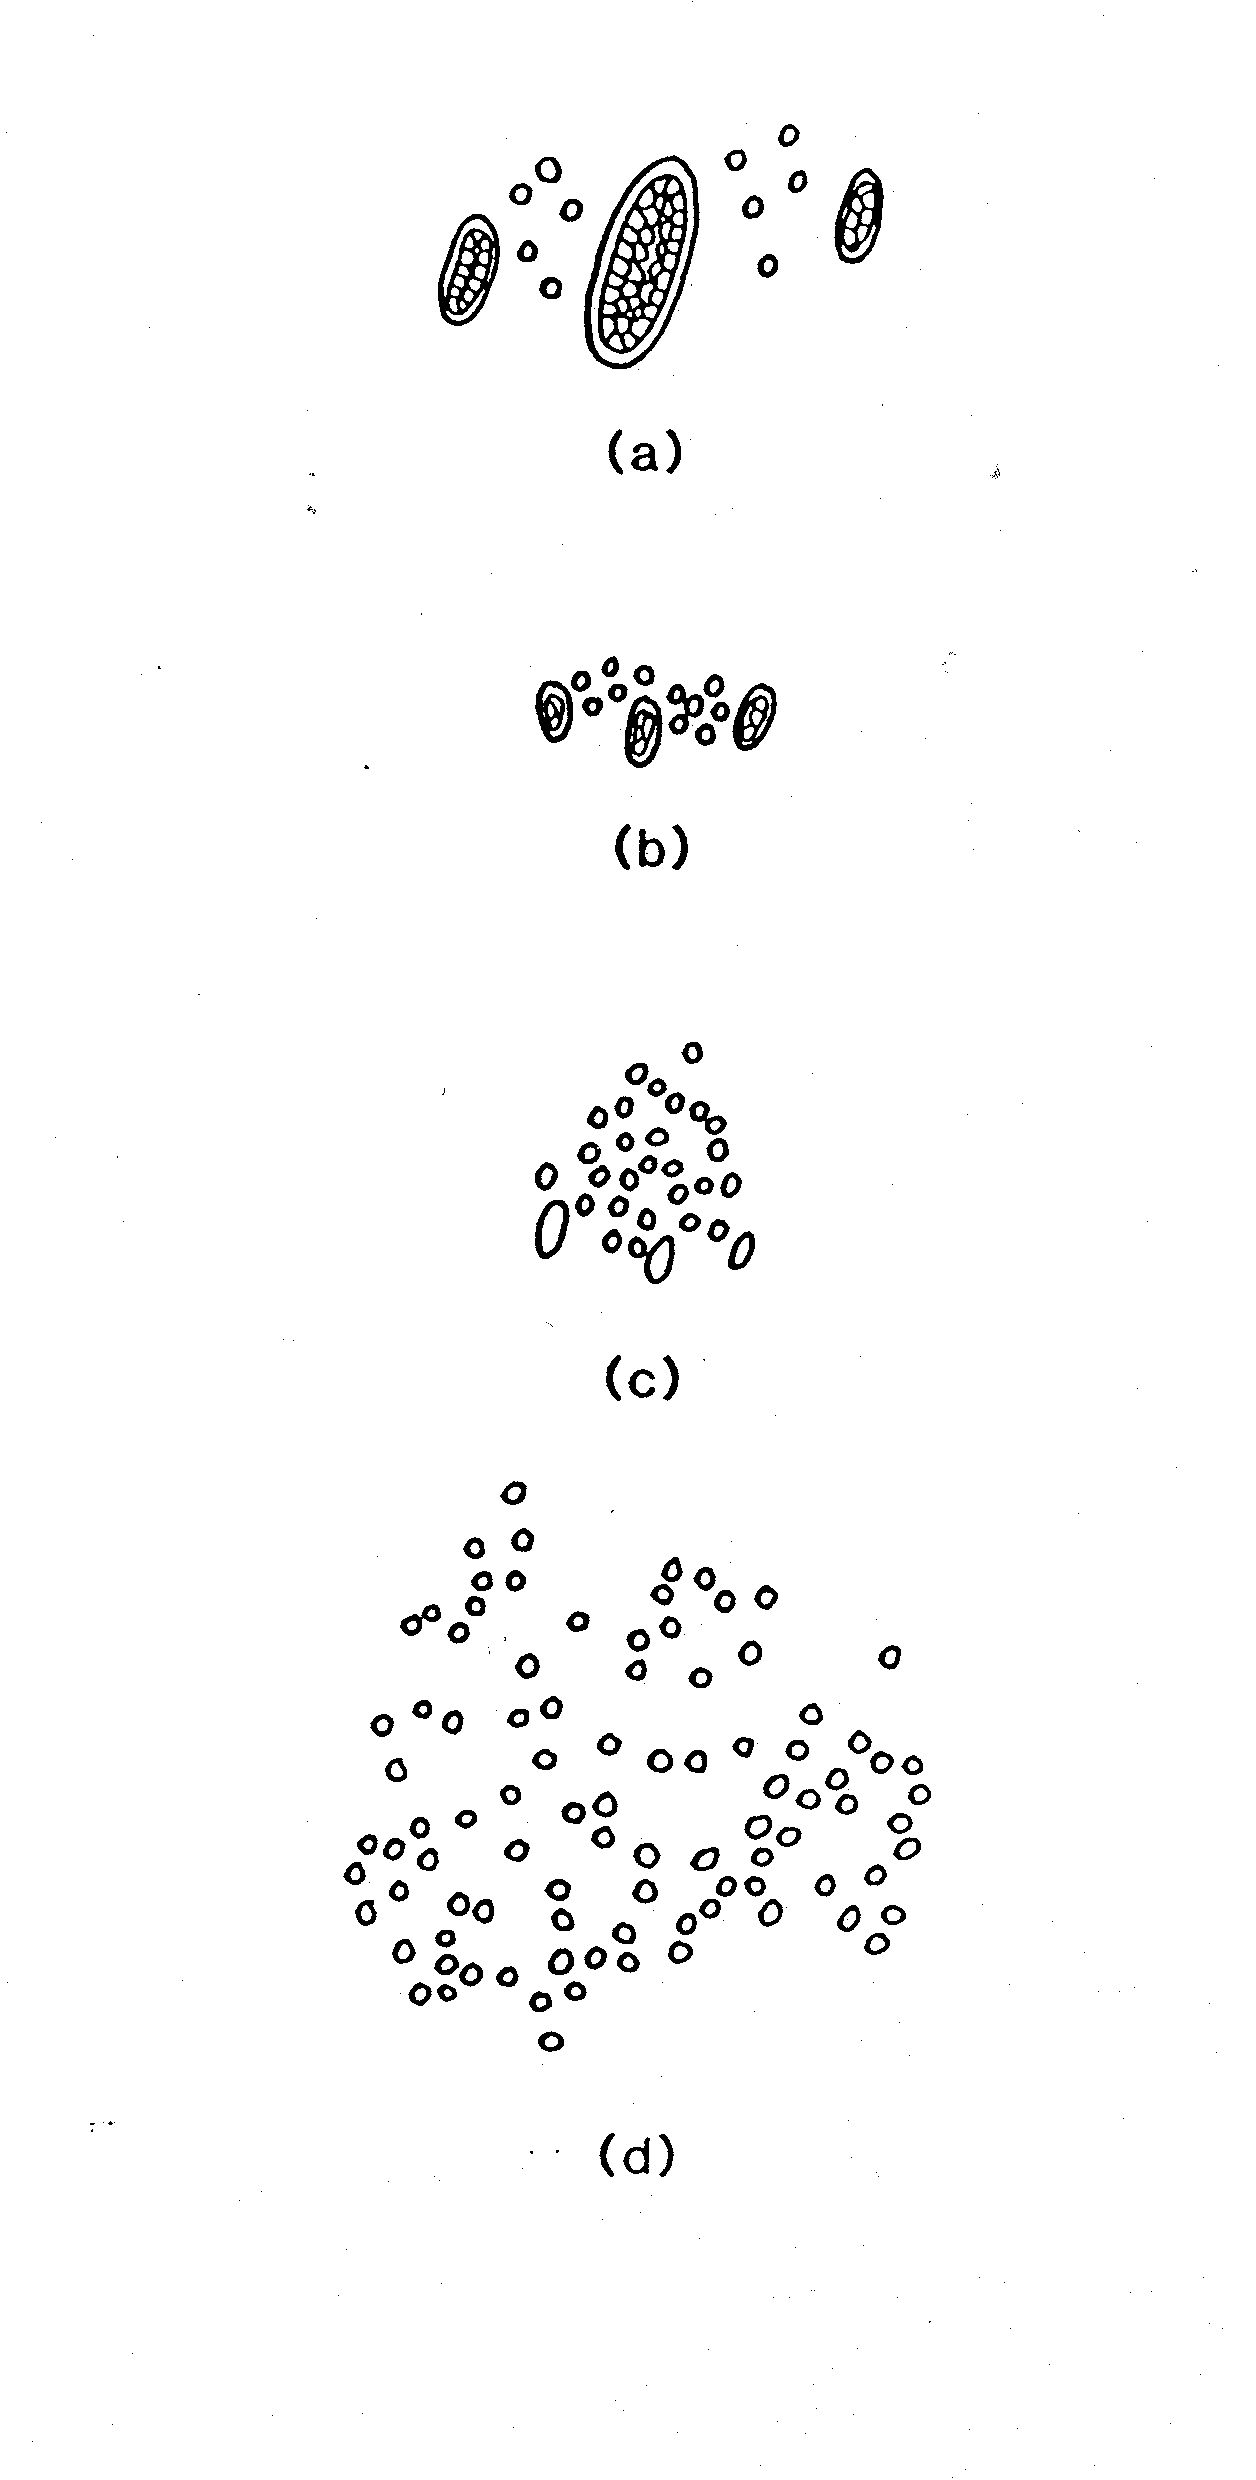
\includegraphics[width=0.8\textwidth, trim = 0 90 0 130]{images/fig7.png}
  \caption{ Tracings of fibre outlines showing changes in follicle group
    arrangement, fibre diameter and medullation through the four
    stages of Merino evolution described in Table 1.  (a) wild sheep,
    (b) primitive domestic sheep, (c) ancient fine/medium wool,
    (d) true fine wool.  Magnification x ....}
  \label{fig:7}
\end{figure}

%\end{document}
